%LaTeX SAMPLE FILE FOR PAPERS OF CDAM

% LaTeX 2e
\documentclass[12pt]{article}

% Delete when translated
\usepackage[T2A]{fontenc}

\usepackage{graphicx}
\usepackage{epsfig}
\usepackage{cite}
\usepackage{amsmath,amssymb,amsfonts,amsthm}
\usepackage[boxed]{algorithm2e}
\usepackage{caption}
\usepackage{wrapfig}
%\usepackage{subfig}
\usepackage{subcaption}
\usepackage{upgreek}
\usepackage{adjustbox}
\usepackage{pbox}
\usepackage{index}
\usepackage{color}
\usepackage{makecell}
\usepackage{multirow}
\usepackage{bbm}
\usepackage{lastpage}
\usepackage{longtable}
\usepackage{changepage}

% LaTeX 2.09
%\documentstyle[12pt]{article}

%%%%%%%%%%%%%%%%%%%%%%%%%%%% paper layout %%%%%%%%%%%%%%%%%%%%%%%%%%%%%%
\hoffset=-1in
\voffset=-1in
% Please, don't change this layout
\parindent=6mm
\topskip=0mm
\topmargin=30mm
\oddsidemargin=27.5mm
\evensidemargin=27.5mm
\textwidth=155mm
\textheight=237mm
\headheight=0pt
\headsep=0pt
\footskip=2\baselineskip
\addtolength{\textheight}{-\footskip}

\providecommand{\keywords}[1]
{
  \vspace{2mm}\hspace{20pt}\textbf{\textit{Keywords:}} #1
}

\providecommand{\abskeyw}[2]
{
  \begin{small}
    \begin{adjustwidth}{10mm}{10mm}
      \vspace{1mm}\hspace{20pt}#1

      \keywords{#2}
    \end{adjustwidth}
  \end{small}
}

\newcommand{\tX}{\mathsf{X}}
\newcommand{\bfX}{\mathbf{X}}
\newcommand{\calX}{\mathcal{X}}
\newcommand{\calT}{\mathcal{T}}
\newcommand{\calH}{\mathcal{H}}
\newcommand{\rmH}{\mathrm{H}}
\newcommand{\iu}{\mathrm{i}}

\theoremstyle{definition}
\newtheorem{definition}{Definition}

\theoremstyle{remark}
\newtheorem{remark}{Remark}

\begin{document}

%%% Title section
\begin{center}
  {\Large\bf TENSORS FOR SIGNAL AND FREQUENCY ESTIMATION IN
  SUBSPACE-BASED METHODS: WHEN THEY ARE USEFUL?}\\\vspace{2mm} {\sc N.A.
  Khromov$^1$, N.E. Golyandina$^2$}\\\vspace{2mm}
  {\it $^{1}$University ...\\
    $^{2}$Institute  ...\\
  City, STATE\\} e-mail: {\tt $^1$ivanov@yandex.ru,
  $^2$petrov@google.com}

  \abskeyw{Abstract text.}{comma, separated, keywords, minimum 3,
  maximum 5}
\end{center}

\section{Introduction}

Intro text...

\section{Алгоритмы}
\subsection{Тензоры вложения}
$\tX = (x_1, x_2, \ldots, x_N)$ --- (одноканальный) временной ряд
длины $N$, $x_n \in
\mathbb{C}$.
\begin{definition}[Оператор вложения временного ряда в тензор]
  Оператором вложения временного ряда в тензор с длинами окна $I$ и $L$:
  ${1< I,L < N},\, {I + L < N + 1}$
  будем называть отображение $\calT_{I,L}$, переводящее ряд $\tX$ в
  тензор $\calX \in \mathbb{C}^{I\times L \times J}$ \linebreak
  (${J= N - I - L + 2}$)
  по правилу $\mathcal{X}_{ilj}=x_{i+l+j-2}$, где $i\in \overline{1:I},\, l
  \in\overline{1:L},\, j \in\overline{1:J}$.
\end{definition}

$\tX = (\tX^{(1)}, \tX^{(2)}, \ldots, \tX^{(P)})$ --- $P$-канальный
временной ряд, состоящий из $P$ одноканальных временных рядов, также
называемых каналами.
\begin{definition}[Оператор вложения многоканального ряда в тензор]
  Оператором вложения многоканального ряда в тензор с длиной окна $L$:
  ${1< L < N}$ будем называть отображение $\calT_{L}$, переводящее $P$-канальный
  ряд $\tX$ в тензор $\calX \in \mathbb{C}^{L\times K \times P}$ \linebreak
  (${K = N - L + 1}$)
  по правилу $x_{l+k-1}^{(p)}$, где $l \in \overline{1:L},\, k \in
  \overline{1:K},\, p \in \overline{1:P}$.
\end{definition}

Визуализации применения вложения к одноканальному и многоканальному
рядам представлены
на картинках~\ref{fig:1d_injection},~\ref{fig:pd-injection}.
\begin{figure}[!ht]
  \centering
  \subfloat[][Результат применения оператора вложения к одноканальному
  временному ряду.]{
    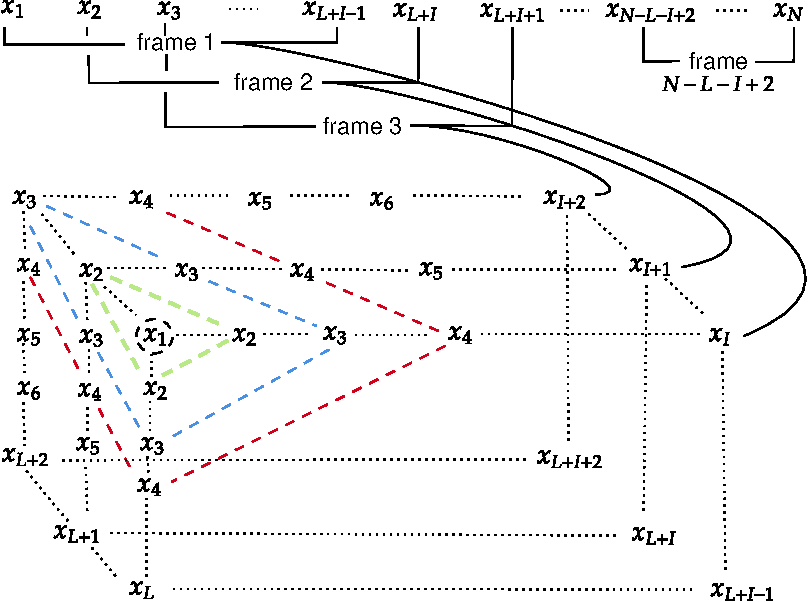
\includegraphics[width=0.45\textwidth]{img/tens-injection-wide.pdf}
  \label{fig:1d_injection}} \qquad
  \subfloat[][Результат применения оператора вложения к многоканальному
  временному ряду.]{
    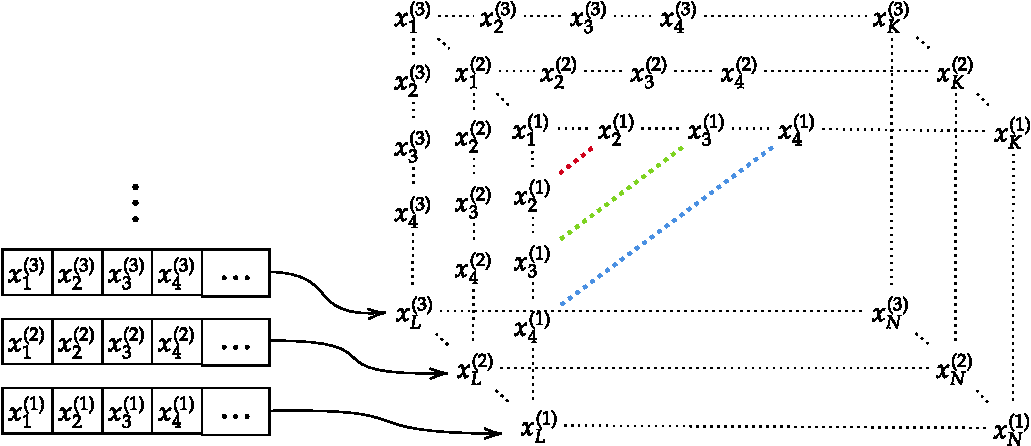
\includegraphics[width=0.45\textwidth]{img/mssa_injection_new.pdf}
    \label{fig:pd-injection}
  }
  \caption{Визуализации результатов применения операторов вложения
  рядов в тензоры.}
\end{figure}

\subsection{Методы для выделения сигнала из временных рядов}
В алгоритме~\ref{alg:hossa} представлен метод HO-SSA для выделения сигнала из
одноканального временного ряда.
\begin{algorithm}[!ht]
  \caption{HO-SSA for signal extraction.}\label{alg:hossa}
  \KwData{$\tX$, $I,L: 1< I,L < N,\, I + L < N + 1$, $R_1 \in \overline{1:I}$,
  $R_2 \in \overline{1:L}$,\\\hspace{36pt}$R_3 \in \overline{1:J}$.}
  \KwResult{$\widetilde{\tX}$ --- оценка сигнала $\tX.$}
  \begin{enumerate}
    \item \textbf{Вложение:} построение $\calX=\calT_{I, L}(\tX)$
      \label{algstep:ssa-inj}\;
    \item \textbf{Разложение:} применение HOSVD или HOOI к $\calX$
      \label{algstep:ssa-decomp}
      \begin{equation*}
        \widehat{\mathcal{X}}=\sum_{i=1}^{R_1} \sum_{l=1}^{R_2} \sum_{j=1}^{R_3}
        \mathcal{Z}_{ilj} U^{(1)}_{i}
        \circ U^{(2)}_{l} \circ U^{(3)}_{j};
      \end{equation*}
    \item \textbf{Восстановление:} усреднение тензора
      $\widehat{\mathcal{X}}$ вдоль
      плоскостей $i+l+j=\operatorname{const}$,
      в результате чего получается оценка сигнала $\widehat{\tX}$.
  \end{enumerate}
\end{algorithm}
\begin{remark}
  Применение алгоритма~\ref{alg:hossa} с такими параметрами длин
  окна, что размер одного любого направления тензора вложения равен
  1, сводит алгоритм к базовому методу SSA, так как применение HOSVD или HOOI
  к тензору с двумя направлениями (матрице) совпадает с применением SVD.
\end{remark}

В алгоритме~\ref{alg:homssa} представлен метод HO-MSSA для выделения сигнала из
многоканального временного ряда.
\begin{algorithm}[!ht]
  \caption{HO-MSSA for signal extraction.}\label{alg:homssa}
  \KwData{$\tX = \left(\tX^{(1)}, \ldots, \tX^{(P)}\right)^{\mathrm{T}}$,
    $L: 1< L < N$, $R_1 \in \overline{1:L}$,
  $R_2 \in \overline{1:K}$, $R_3 \in \overline{1:P}$ ($K = N-L+1$).}
  \KwResult{$\widetilde{\tX} = (\widetilde{\tX}^{(1)},
      \widetilde{\tX}^{(2)}, \ldots,
  \widetilde{\tX}^{(Q)})$ --- оценка сигнала $\tX$.}
  \begin{enumerate}
    \item \textbf{Вложение:} построение $\calX=\calT_{L}(\tX)$
      \label{algstep:mssa-inj}\;
    \item \textbf{Разложение:} применение HOSVD или HOOI к $\calX$
      \label{algstep:mssa-decomp}
      \begin{equation*}
        \widehat{\mathcal{X}}=\sum_{l=1}^{R_1} \sum_{k=1}^{R_2} \sum_{p=1}^{R_3}
        \mathcal{Z}_{lkp} U^{(1)}_{l}
        \circ U^{(2)}_{k} \circ U^{(3)}_{p};
      \end{equation*}
    \item \textbf{Восстановление:} сечения $\mathring{\calX}_{\cdot\cdot p}$
      усредняются вдоль побочных диагоналей $l + k = \operatorname{const}$ для
      получения оценок $\widetilde{\tX}^{(p)}$.
  \end{enumerate}
\end{algorithm}
(\emph{Возможно можно сократить запись, если написать, что шаг 1 такой
    же как и в одномерном
    алгоритме, но оператор вложения другой, шаг 2 полностью совпадает,
шаг 3 обратный шагу 1?}.)
\begin{remark}
  Применение алгоритма~\ref{alg:homssa} к одноканальному
  ряду также даёт базовый алгоритм SSA.
\end{remark}

\begin{remark}
  Если в алгоритме~\ref{alg:homssa} слои третьего направления
  траекторного тензора соединить в матрицу по столбцам (получится
  матрица, состоящая из $P$ блоков-матриц $L\times K$), применить к
  ней SVD, построить приближение этой матрицы по первым $R$
  компонентам разложения, и затем применить антидиагональное
  усреднение к каждму блоку-матрице, то получится метод MSSA.
\end{remark}

\subsection{Методы для оценки параметров сигнала.}
Пусть $P$-канальный временной ряд (возможно $P=1$) имеет вид
\begin{gather*}
  \tX = (\tX^{(1)}, \tX^{(2)}, \ldots, \tX^{(P)}),\\
  \tX^{(p)} = (x_1^{(p)}, x_2^{(p)}, \ldots, x_N^{(p)}), \quad
  p=\overline{1:P},\\
  x_n^{(p)}= \sum_{r=1}^{R} a_r^{(p)} e^{\alpha_r n} e^{\iu\left(2\pi
  \omega_r n + \varphi_r^{(p)}\right)},
\end{gather*}
где параметрами модели являются амплитуды $a_j^{(p)} \in
\mathbb{C}\setminus\{0\}$, фазы ${\varphi_j^{(p)} \in [0, 2\pi)}$,
частоты $\omega_j\in [0, 1/2]$ и степени затухания $\alpha_j \in \mathbb{R}$.
Алгоритм HO-ESPRIT, оценивающий частоты и степени затухания ряда,
определяется следующим образом.
После шага~\ref{algstep:mssa-decomp} алгоритма~\ref{alg:homssa} (или
шага~\ref{algstep:ssa-decomp} алгоритма~\ref{alg:hossa} при $P=1$)
строится матрица $\mathbf{U} = \mathbf{U}_d = \left[U_1^{(d)} :
U_2^{(d)}:\ldots : U_{R_d}^{(d)}\right]$ для некоторого $d\in \{1, 2,
3\}$, и решается уравнение
\begin{equation*}
  \mathbf{U}^{\uparrow}=\mathbf{U}_{\downarrow}\mathbf{Z}
\end{equation*}
относительно матрицы $\mathbf{Z}$, где запись $\mathbf{U}^{\uparrow}$ означает
матрицу $\mathbf{U}$ без первой строки, а $\mathbf{U}_{\downarrow}$
--- без последней.
$R$ наибольших собственных чисел матрицы $\mathbf{Z}$ считаются
оценками $\lambda_r = e^{\alpha_r + 2\pi\iu \omega_r}$, из которых
можно получить параметры $\alpha_r$ и $\omega_r$.
Базовые алгоритмы ESPRIT, использующие траекторную матрицу и SVD
можно получить из HO-ESPRIT аналогично тому, как из HO-SSA и HO-MSSA
можно получить базовые SSA и MSSA.


\subsection{Dstack модификация ESPRIT}
При большой длине ряда $N$ вычисление HOSVD (SVD) траекторного
тензора (матрицы) может быть довольно трудоёмкой задачей.
Одним из способов бороться с этой проблемой является модификация
алгоритма EPSRIT: HTLSDstack (HTLS --- другое название ESPRIT).
Метод HTLSDstack разработан для одноканальных временных рядов.
(\emph{Возможно здесь вставить фразу, что он обобщается на
многоканальные ряды, но такой случай мы рассматривать в работе не будем.})

Метод заключается в том, чтобы по одноканальному временнмоу ряду
$\tX = (x_1, x_2, \ldots, x_N)$ построить многоканальный ряд
$\tX_D = (\tX^{(1)}, \tX^{(2)}, \ldots, \tX^{(D)})$,
где $D$ - некоторый параметр (предполагается, что $N$ делится на $D$ нацело),
а элементы рядов $\tX_D^{(d)}$ получаются из оригинального ряда by
decimating the time series by factor D.
Другими словами, $x_m^{(d)} = x_{(m-1)D + d}$, где $m \in \overline{1:(N/D)}$.
Затем к полученному многоканальному ряду применяется многоканальный
вариант метода HO-ESPRIT или ESPRIT.
По Nyquist-Shannon sampling theorem, можно увеличивать sampling time
interval $\Delta t$ в $D$ раз с сохранением всех частот в сигнале, пока
сохраняется равенство $\max\limits_{r}\left|\omega_r\right| < 1 / (2
D \Delta t)$.


\section{Сравнение тензорных методов с матричными}
Тут привести какие-нибудь таблички и, может, графики.
%% please make bibitems content in a style below !!!
%% papers with "free style" bibitems content will be rejected !!!

\begin{thebibliography}{10}

  \bibitem{Papy2005}
  Papy~J.M., De~Lathauwer~L., Van~Huffel~S.~(2005).
  Exponential data fitting using multilinear algebra: the
  single-channel and multi-channel case.
  {\sl Linear Algebra with Applications}. Vol.~{\bf 12}, Num.~{\bf 8},
  pp.~809-826.

  \bibitem{Papy2009}
  Papy~J.M., De~Lathauwer~L., Van~Huffel~S.~(2009).
  Exponential data fitting using multilinear algebra: the decimative case.
  {\sl Journal of Chemometrics}. Vol.~{\bf 23}, Num.~{\bf 7-8},
  pp.~341-351s.

  \bibitem{paper}
  Jacobs~P.A., Lewis~P.A.W.~(1983). Stationary Discrete
  Autoregressive-Moving Average
  Time Series Generated by Mixtures. {\sl Journal of Time Series
  Analysis}. Vol.~{\bf 4}, Num.~{\bf 1},
  pp.~19-36.

  \bibitem{book}
  Johnson~N.L., Kotz~S., Balakrishnan~N.~(1997). {\sl Discrete
  Multivariate Distributions}. Wiley: New York.

  \bibitem{web}
  Worldometers.info [Electronic resource] Mode of access:
  \texttt{https://www.worldometers.info/coronavirus.} Date of access:
  27.02.2022.

\end{thebibliography}


\end{document}
